\chapter{Stop and think: Exploring mobile notifications to foster reflective practice on meta-learning} 

\vfill
This chapter explores the effectiveness of mobile notifications to foster reflection on meta-learning by presenting the results of two studies: 1) a formative study with 37 secondary school students offering a daily reflection and reporting exercise about their learning experience during the day; 2) an experiment involving 60 adults to read an eBook on energy-efficient driving for one hour. During that time, the participants received mobile notifications inviting them to reflect in-action. On the one hand, the results from the first study show that students do not have a habit of seeing themselves as learners and developing a \em ''professional'' \em awareness about their daily activity at work/school. On the other hand, the second study explores the effects of different notification types on knowledge gain and motivation. Results envision a higher knowledge gain and motivation for the group assigned with the least complex interactions with mobile devices during the reflection exercise.
\vspace{3em}

This chapter is published as: 
Tabuenca, B., Kalz, M., Ternier, S., \& Specht, M. (2014). Stop and think: Exploring mobile notifications to foster reflective practice on meta-learning. \em IEEE Transactions on Learning Technologies\em . Special Issue on Seamless, Ubiquitous, and Contextual Learning. 1�12. doi:10.1109/TLT.2014.2383611

\clearpage

\section{Introduction}

Based on current trends \citep{Publishing2011}, it is estimated that 84 percent of today�s young people in OECD countries will complete upper secondary education over their lifetimes. This period consolidates students� basic skills and knowledge towards a successful transition to either an academic or a vocational pathway. While graduation rates give an indication of the extent to which education systems are succeeding in preparing students to meet the labour market�s minimum requirements, they do not capture how the students have developed an identity as learners. The acquisition of such an identity, and the associated reflective transversal skills, grow in importance in a \em ''lifelong learning society'' \em  \citep{EuropeanComission2005}. In the formal education system it is a challenge to find ways to provide students with opportunities to mentally evoke what they have learned throughout the day, so that this experience can be turned into a deliberate object of attention and reflection.

\em Learning to learn  \em and \em Digital competence  \em are highlighted as two of the eight key competences for lifelong learning in the European Reference Framework \citep{EuropeanCommission2007}. The proliferation of wirelessly-networked technologies facilitates the scaffolding of \em seamless learning spaces \em \citep{Chan2006} as an approach for continuing learning experiences across different scenarios, and emerging from the availability of one device or more per person. \cite{Biggs1985} defines meta-learning as an awareness and understanding of the phenomenon of learning itself as opposed to subject knowledge. Hereby we conceive meta-learning activities as the increase of knowledge and motivation on learning when triggered by introspective episodes of reflection on user�s own learning. Hence the present chapter explores different instantiations of notifications received on mobile devices with the aim to foster reflective practice for meta-learning measuring the variations in dependent variables of knowledge and intrinsic motivation.

Reflection is the practice to become aware of an implicit knowledge base and to learn from experience \citep{Schon1983}. Sch\"on coined the terms \em reflection in-action \em as the reflective practice performed while doing an activity to optimize the immediately following action, and, \em reflection on-action \em as the reflective practice performed when the activity has finished in order to review, analyse, and evaluate the situation and gain insight for improved practice in the future.

Previous work on reflection amplifiers in-action suggests that regular changes between meta-cognitive and content focus, lead to more awareness and self-regulative competences in the learning process \citep{Bannert2009,Verpoorten2012}. Reflection amplifiers are compact and well-considered prompting approaches that offer learners structured opportunities to examine and evaluate their own learning \citep{Verpoorten2009}. They are present as structured and repeated introspective episodes, offered in the course of action and meant to make learning visible. The effectiveness of mobile notifications to foster reflective practice on learning (reflection on-action) has not been explored yet. Recent research suggests that mobile notifications by students produce distracting effects \citep{Fried2008,Kraushaar2010}. Nonetheless, notifications received on mobile devices have also resulted in a positive impact, suggesting that the intervention is able to improve students� self-regulated learning effort. The study from \cite{Goh2012a} used persuasive SMS interventions on undergraduate students for 12 weeks, showing that students who received SMS intervention performed better than students who did not receive SMS intervention. \cite{Cavus2009} investigated the effects in knowledge and enjoyment of sending SMSs with English vocabulary to 45 first-year undergraduate students concluding that students enjoyed and learned new words with the help of their mobile phones. Similar, \cite{Thornton2005} used more elaborated notifications in the form of emails to teach English vocabulary lessons to university students concluding that students that received the mobile email learned more than those that received web-based email. \cite{Uzunboylu2009} implemented multimedia messages to increase awareness on environmental concerns. Measures of enjoyment, knowledge or awareness have been the focus of previous research.

This chapter presents two studies evaluating approaches to stimulate learners� capacity of reflection by making \em what they learn \em  a deliberate object of attention \citep{Watkins2001}. The research is embedded into a larger project focusing on mobile support for lifelong learning \citep{Tabuenca2013,TabuencaCAA2014,Tabuenca2014d}. More specifically, in this work we have focused on the use of notifications instantiated in mobile devices for lifelong learning support. Research on notification and prompting for reflection suggest different strategies for reflection on-action and in-action. This work advances the research on mobile notifications and reflective practice presenting two studies:
\begin{itemize}
\item A formative study aimed to reflect on-action. This study was carried out during two school days and two days off, in which 37 college pupils were prompted via mobile SMS notification for a daily reflection and reporting exercise about how they have learned during the day (intensity and channels).
\item An experimental study aimed to reflect in-action. In this study, 60 university employees were invited to read an eBook on energy-efficient driving. During that time, they were prompted via mobile notifications to reflect and report on what they had learned.
\end{itemize}
The following sections introduce both experiments by mapping the goal of the research to existing gaps that need to be covered. The results are discussed and important research questions are raised.

\subsection{How to design mobile notifications for student reflection support}
The first study presented in this chapter transposes \em reflection amplifiers \em \citep{Verpoorten2009} to mobile (meta-)learning, after-school setting and analytical scrutiny onto one�s learning day.  In this study, students have been assigned to reflect about the learning affordances offered to them throughout the day. Three main research questions have guided this formative study:
\begin{enumerate}
\item How will students respond to invitations to reflect on personal learning sent on their own device and outside the school hours (participation)?
\item What insight does this sampling of experience bring regarding how learning takes place in students� today common life (channels of learning and perceived intensity)?
\item What effects of these structured episodes of introspective reflection can be pinpointed on dimensions of learning (familiarity, appreciation, perceived learning, account of the learning experience)?
\end{enumerate}
In a second experiment, variations of mobile notifications prompting users to reflect in-action have been explored, and the effects on knowledge gain and motivation have been quantified.
On the one hand, thinking aloud \citep{Nielsen2002} and sampling of experiences \citep{Hektner2007} have been pinpointed as effective approaches to foster reflective practice on learning. The majority of the studies sampling experiences with educational implications have involved children and adolescents \citep{Hektner2007}. Hence, this experiment has been performed with adults. On the other hand, \cite{Wong2011d} identify ten seams by which learning experiences are disrupted and for which mobile seamless learning technology has to find new solutions. One of them is \em''the combined use of multiple device types'' \em. In many cases it is presumed that learners interact only through a single channel or device. However, the technological framing can vary from single device interaction to the presence of multiple devices with different characteristics and capabilities that are used simultaneously. Likewise, the proliferation of tagged objects and the incorporation of tag readers (i.e.QR codes, NFC tags) to mobile devices are facilitating the exchange of educational content across devices.
This experiment explores variations of mobile notifications for adults sent with the aim to foster reflective practice in-action while accomplishing a learning activity. This setup contemplates the combined use of multiple devices for learning and has been guided on three main research questions:
\begin{enumerate}
\setcounter{enumi}{3}
\item How do students perceive asynchronous notifications in contrast to user-triggered notifications prompting reflection in-action, and, what effects on knowledge and motivation can be highlighted?
\item What insights can be gained when using mobile notifications prompting the student to actively externalize an exercise of reflection in-action, and, what effects on knowledge and motivation can be highlighted?
\item Which reflection cues are provoked by the spontaneous collection of learning objects with mobile devices, and, what effects on knowledge and motivation can be highlighted?
\end{enumerate}

\section{Study 1: Embedding reflection in everyday activity via SMS notifications}
\subsection{Method}
\subsubsection{Participants}
This study enrolled 37 college students (mean age = 17 years old, 37\% female, 63\% male). An iTunes voucher of 15 EUR rewarded their participation in the experiment. The voucher was delivered to students that completed both the pre-questionnaire and the post-questionnaire.

\subsubsection{Materials}
The formative study aimed to attract every student to perform the reflection exercise, no matter which mobile device they were using. It was decided to use SMSs notifications to make them all aware when the personal response system was ready to accomplish the reflection exercise. Participants that reported to own a phone with Internet connection (67\%) could follow the link in the SMS (See figure \ref{fig:notif_1}a) to directly navigate within the personal response system. Participants without mobile Internet connection (33\%) used alternative devices (personal computers or tablets) to log in via browser navigation of the same URL. The students' personal response system\footnote{Socrative. Multiplatform audience response system. http://www.socrative.com/}  selected for this formative study features multiple-choice questions (figure \ref{fig:notif_1}bc), short text answers, and long text answers. This platform can be accessed from smartphones, tablets, laptops and personal computers. Materials, experimental design and partial results of this study were reported earlier  \citep{Tabuenca2012d}. The current chapter provides additional data (Table \ref{tbl:notif_table2} and dropouts examination) extending the analysis of these results and its implications.
\begin{center}
\begin{figure}[ht]
\centering
	\subfloat[Daily SMS received by students]{
		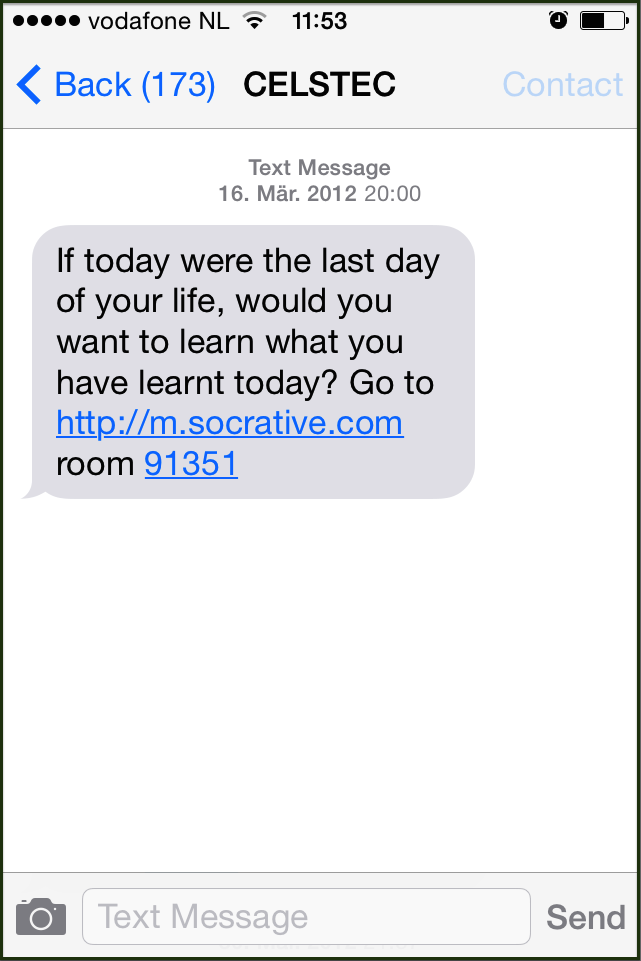
\includegraphics[width=0.3\linewidth]{img/notif_fig1a}
		\label{fig:notif_1a}
	}
	\subfloat[Personal response system: \em What was your main learning channel today? \em]{
		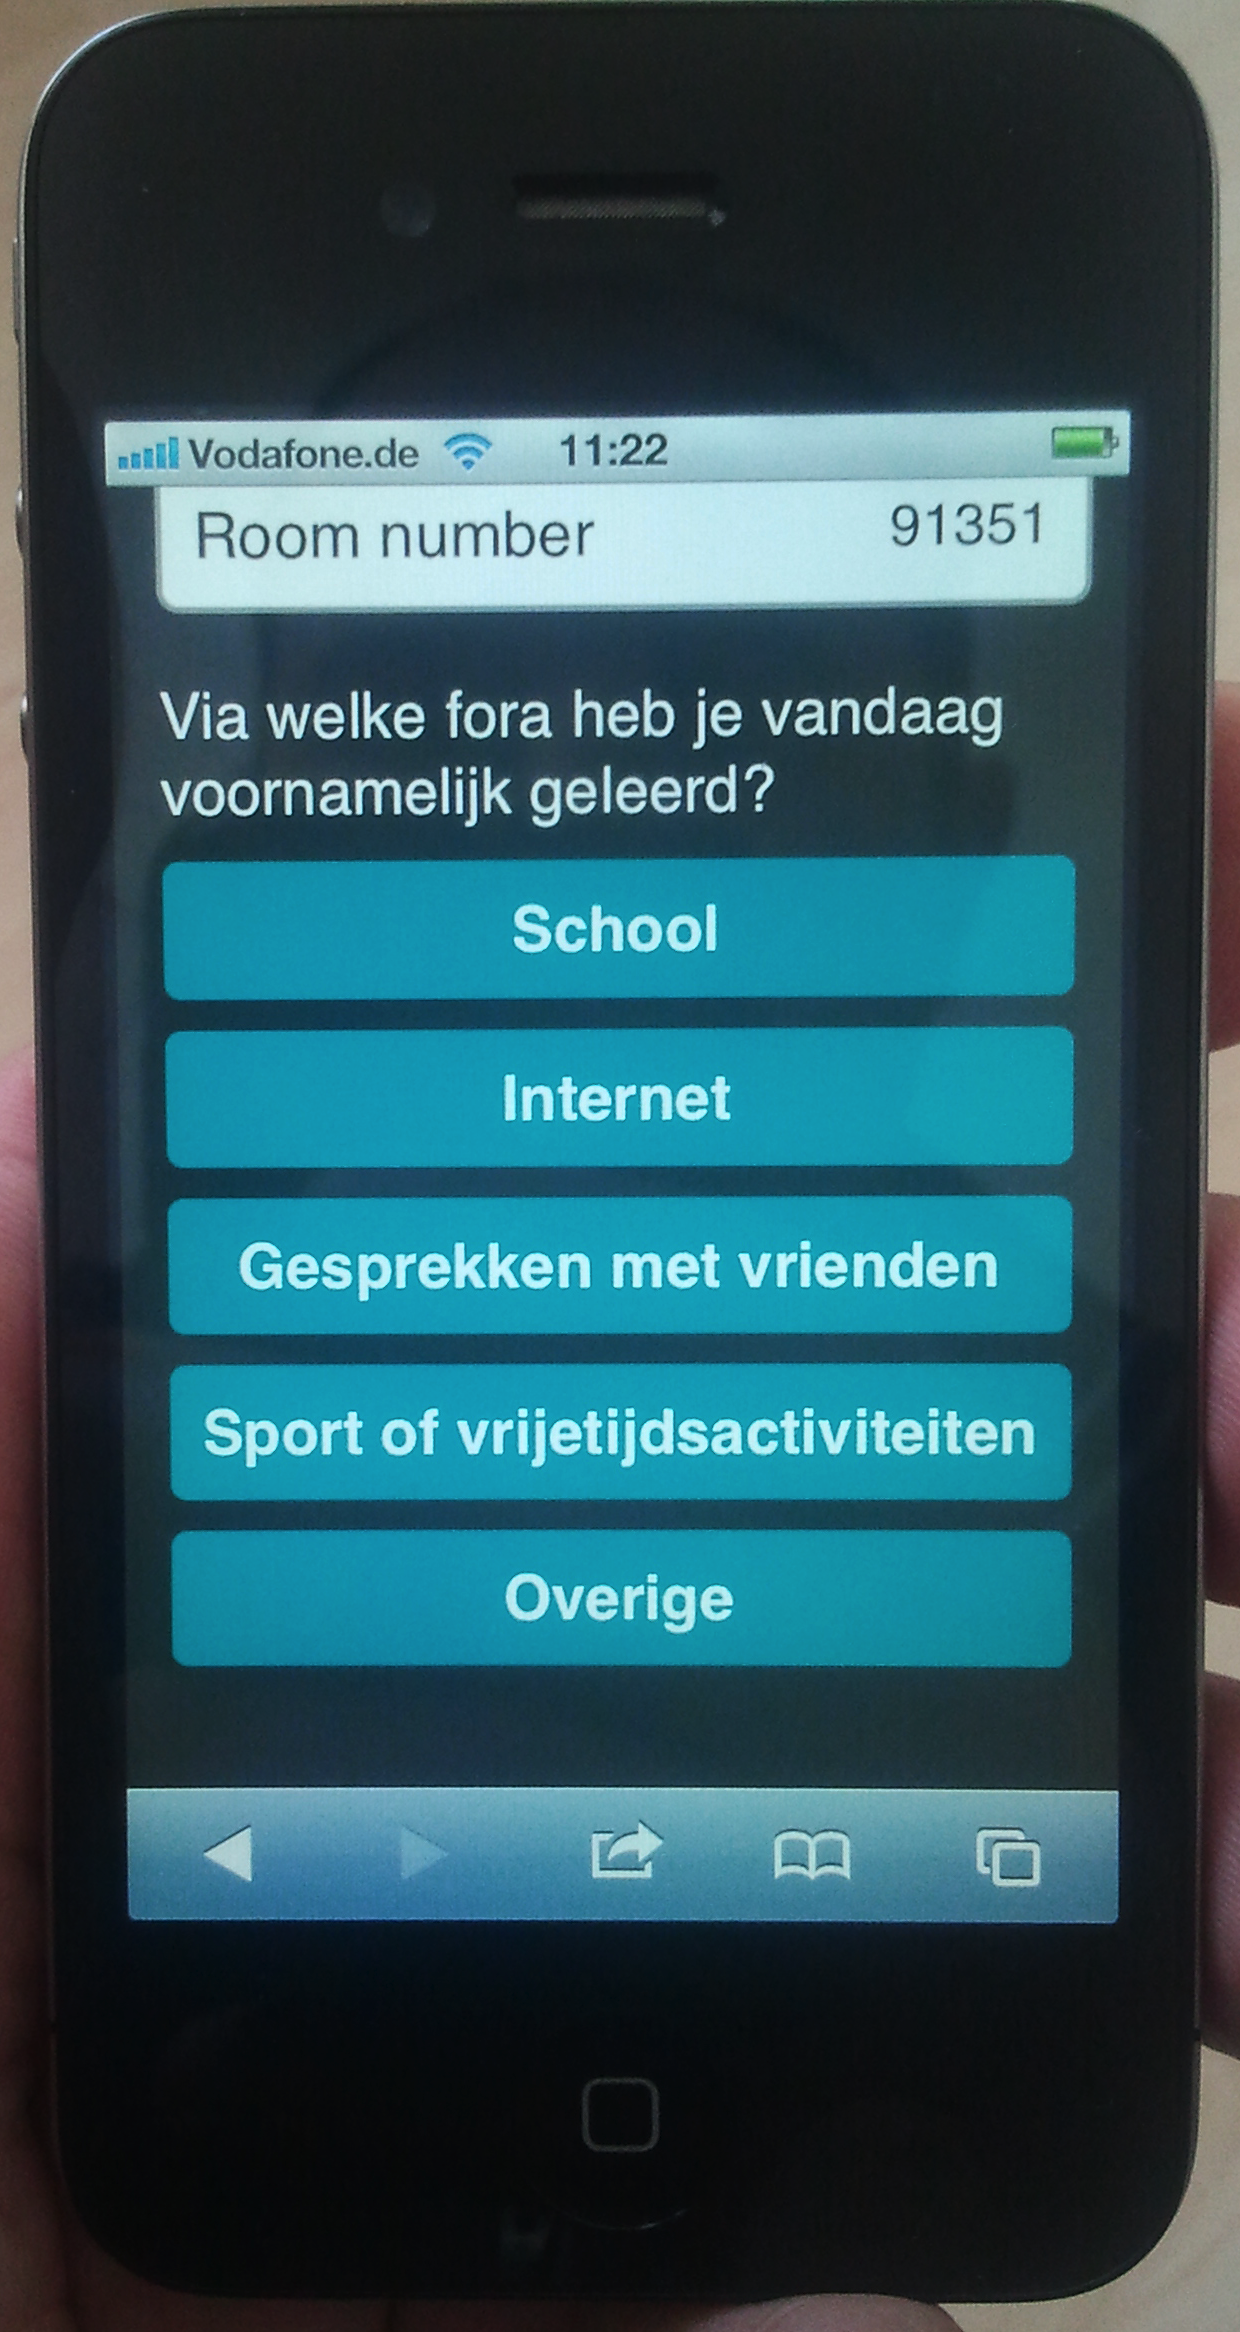
\includegraphics[width=0.3\linewidth]{img/notif_fig1b}
		\label{fig:notif_1b}
	}	
	\subfloat[Personal response system: \em How intense was your learning day? \em]{
		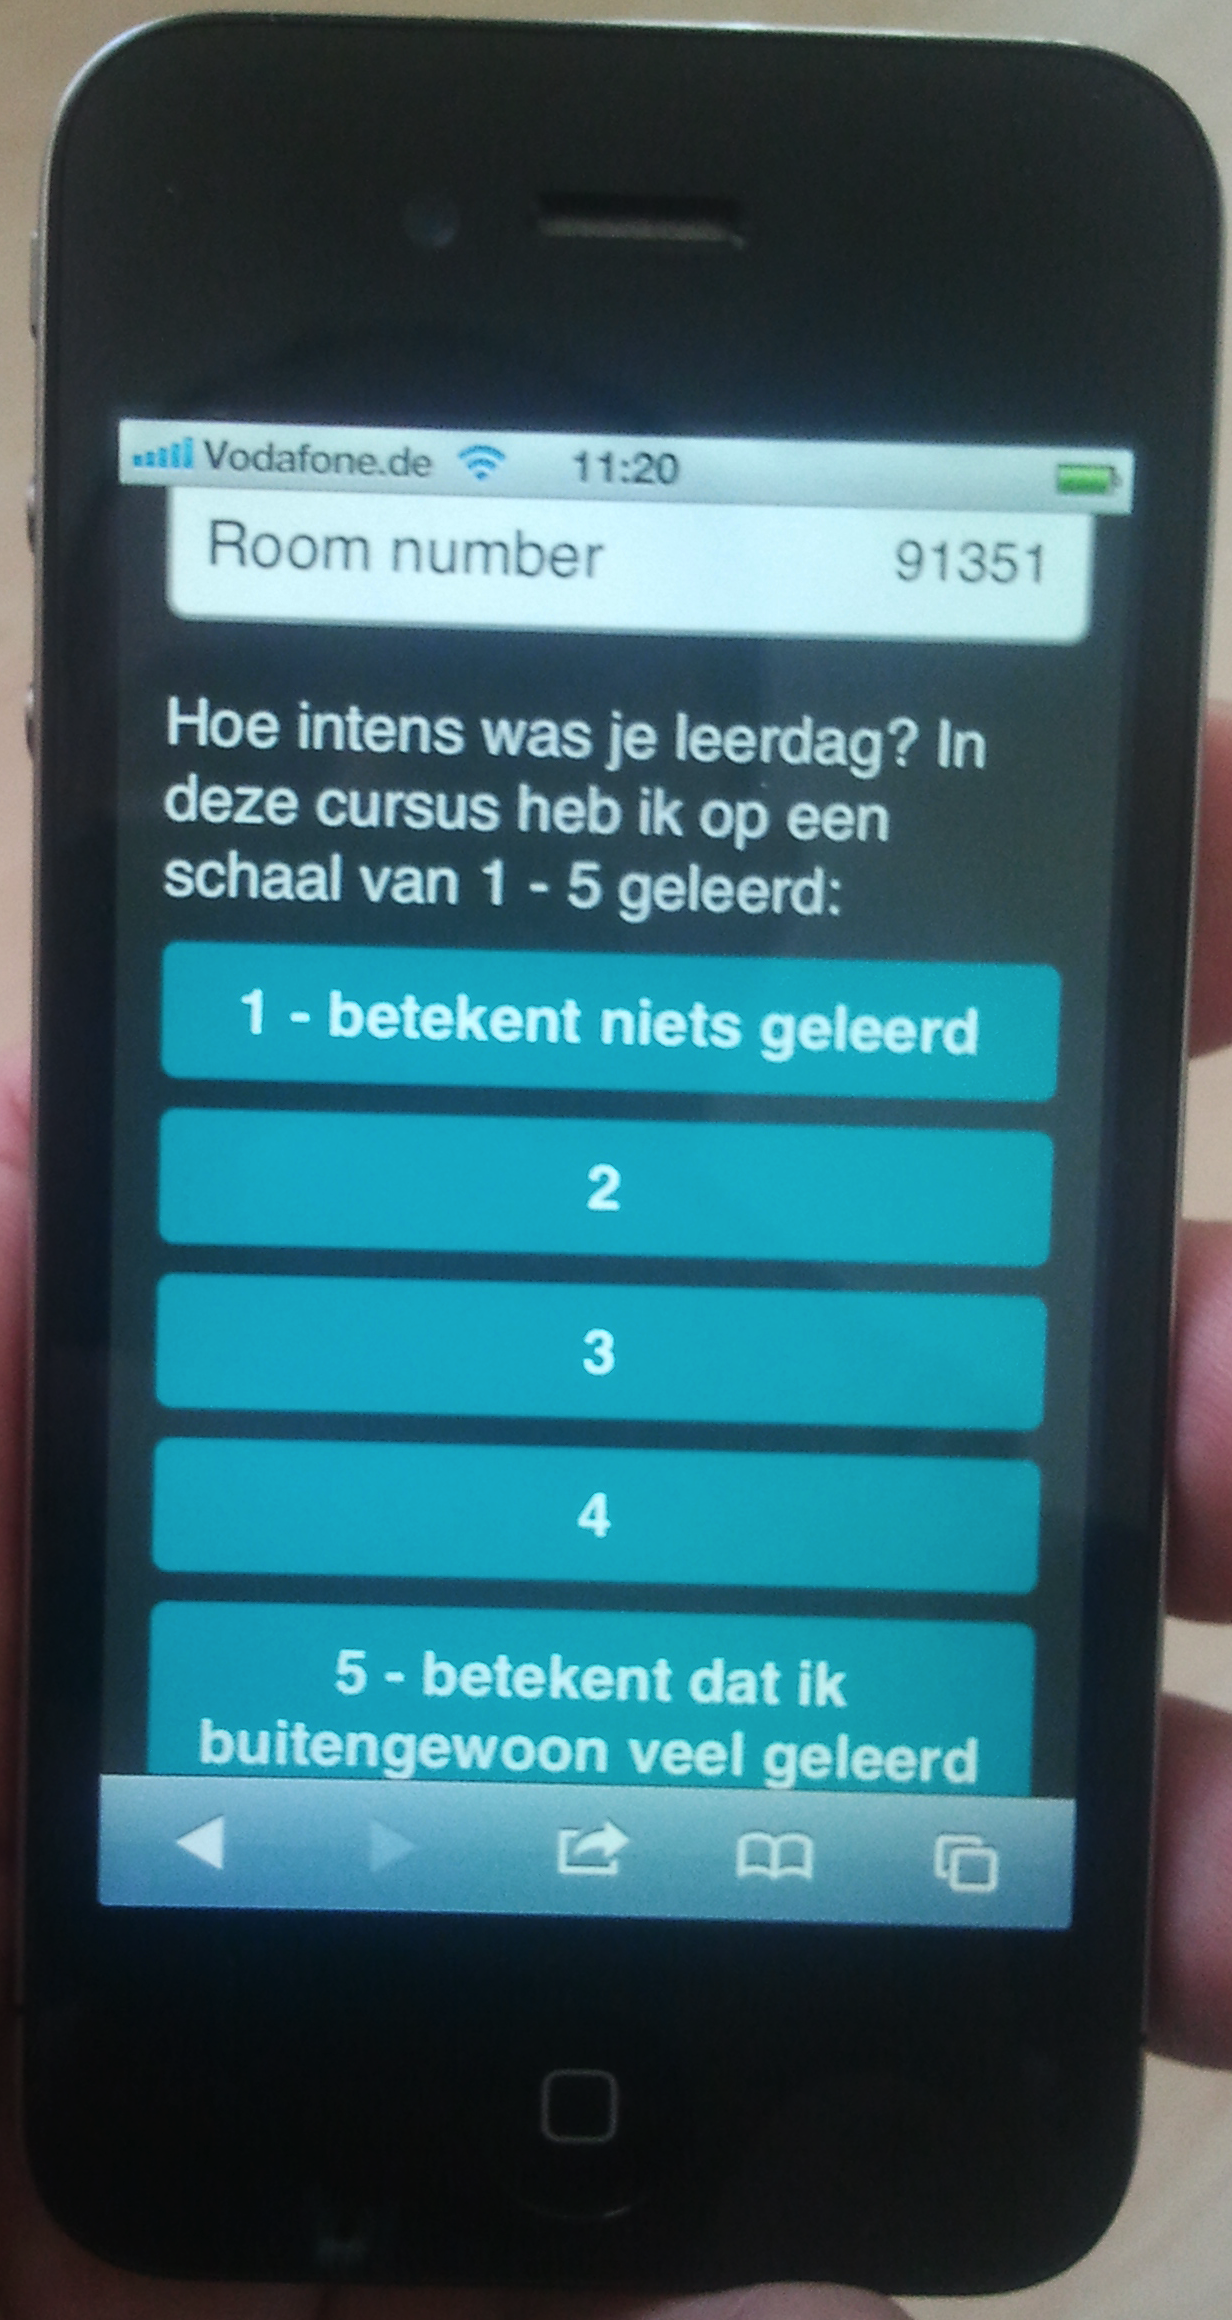
\includegraphics[width=0.3\linewidth]{img/notif_fig1c}
		\label{fig:notif_1c}
	}	
      \caption{Formative study. Notifications fostering reflective practice on-action}
      \label{fig:notif_1}
\end{figure}
\end{center}
\subsubsection{Design}
The design of this study considered the same treatment for all the participants. Regarding the independent variables, this formative study considered three measures:
\begin{itemize}
\item A pre-questionnaire gathered perception of students about the intensity of their learning week and the main channel they use for learning. 
\item A daily mobile questionnaire was the reflection amplifier of the study. It comprised one question about the perceived intensity of the learning day (figure \ref{fig:notif_1c}) and one question about the main channel of learning used during the day (figure \ref{fig:notif_1b}).
\item A post-questionnaire left active during one week served to explore the effects of introspective episodes of reflection on meta-learning defined as awareness and understanding of the phenomenon of learning itself \citep{Biggs1985}. Hence, participants were prompted to reflect and report on \em''What is learning?'' \em, their familiarity with reflective practice, their appreciation of the reflective practice, and their description of the learning experience. Additionally, they were asked to provide an account on their learning channels, and the intensity of their learning during the days of the experiment. The high rate of dropouts motivated the adaptation of a post-questionnaire with the intention to explore the reasons why some students did not take part in the daily reflective exercise.
\end{itemize}

\subsubsection{Procedure}
The study took place during an ''experiment day'' which offered students to discover the work of the Learning Innovation Lab (the authors� workplace) through the participation in empirical experiments. At the end of the day, a presentation provided an overview of mobile technologies for learning. Afterwards, the corresponding author introduced the participants to the exercise to be done in the next 4 days. The formative study was introduced to students as a reflection exercise in which they were supported to improve their awareness of their daily activity as learners. The famous speech of Steve Jobs at the end of the year session at Stanford University\footnote{Jobs, S. (2005). Commencement address delivered at Stanford University, June 12, 2005. Stanford Report. Available in http://www.youtube.com/watch?v=xoUfvIb-9U4}  was used as a stance on the importance to step back and consciously attend to one�s own life and personal identity, here as a learner. The experiment required using both a SMS broadcasting system that would alert them about the reflection moment of the day, and a student response system where they should answer the questions they would be asked. The students completed the pre-questionnaire and a demo from both the SMS functionality and the student response system was performed.

The daily reflection exercise was performed during 4 consecutive days after the presentation of the experiment. This setup was designed to evenly distribute the reflection exercises across two days at school (Thursday to Friday) and two days out of school (Saturday to Sunday). It allowed to encompass the awareness and reflection on both formal and informal learning and to provide contrast to the descriptions of the learning experience. An SMS was sent to students every day at 8 pm alerting them that the student response system was ready to receive answers with their reflections. Students that had smartphone with Internet connection could click the link and perform the reflection exercise within the platform directly on their smartphone device. The virtual classroom enabled the teacher monitor how many students were performing the activity in real time. Finally, the students received an email inviting them to complete the post-questionnaire.

\begin{figure}
     \centering
     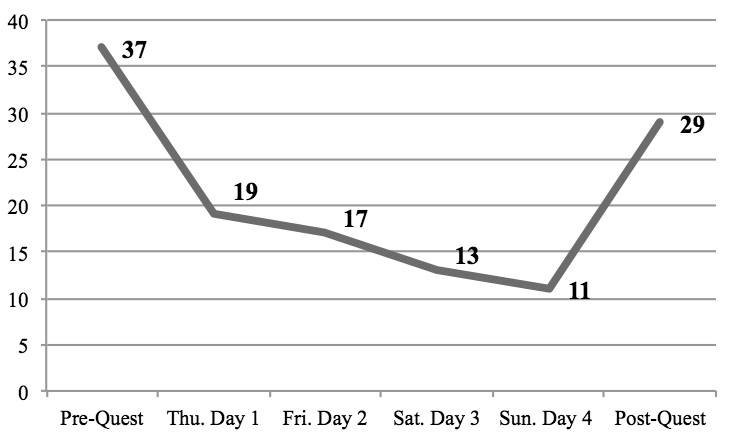
\includegraphics[width=0.7\linewidth]{img/notif_fig2}
     \caption{Evaluation of the participation in the formative study}
     \label{fig:notif_2}
\end{figure}

\subsection{Results}
\subsubsection{Participation}
The first research question aimed to explore student�s willingness to participate in a reflection exercise and to what extent students would react actively to regular invitations to reflect on personal learning experiences sent on their own device and outside the school hours. The decrease in participation (figure \ref{fig:notif_2}) was quite visible in each of the four iterations of the daily questionnaire (mean 2\%), but was not as severe as the dropout rate from the pre-questionnaire to the mere entrance in the daily exercise (48\%). The 29 recorded post-questionnaires comprised both the participative (56\% [n=16]) and the dropouts (44\% [n=13]). In this study, we refer to dropouts as the students that voluntarily decided not to take part in the daily reflection exercise (Day 1 to 4). Dropout students had the chance to get the reward (iTunes voucher) whenever they completed the post-questionnaire for dropouts.

Main invoked reasons for dropouts (n=13) were for 46\% \em''I did not receive any SMS'' \em and 38\% \textit{''I had no internet connection at that moment''}. No respondent selected lack of interest, boredom of the intrusive character of the experiment as justifications for not participation. The SMS monitor tool confirmed the failures delivering the messages: an average of 15\% of the SMS were not delivered, a large majority thereof caused by a wrong phone number given by the students right from the start of the experiment. Additionally, the monitoring tool for teachers of the student response system displayed how many students were connected to the platform filling-out the questionnaire in every moment. From these observations, it can be concluded that the majority of the students reported their answers in the same moment they received the SMS.

\subsubsection{Intensity of the learning day and channels used}
The second research question aimed to gain insights on what this sampling of experience brings regarding how learning takes place in students� life focusing on their channels of learning (figure \ref{fig:notif_1b}). Table \ref{tbl:notif_table1} summarizes the answers given by students both in the pre/post-questionnaires and in the daily reflection exercises. School and Internet were reported as the most important sources of learning.

The post-questionnaire shows that the majority of the participants in the daily reflective exercise reported the school as the main channel of learning during those days. Nevertheless, the majority of the dropouts identified Internet as the main leaning channel.
\begin{table}[h]
  \centering
  \footnotesize
  \caption{Main channels of learning}
  \label{tbl:notif_table1}
  
\begin{tabular}{llllllll}
\thickhline
\textbf{ }								
	& \multicolumn{1}{c}{\textbf{School}}	
	& \multicolumn{1}{c}{\textbf{Internet}}
	& \multicolumn{1}{c}{\textbf{Conversations}}
	& \multicolumn{1}{c}{\textbf{Leisure}}
	& \multicolumn{1}{r}{\textbf{Other}}              
	& \textbf{} 
	& \textbf{} \\ \thickhline
\textbf{Pre-Quest (n=37)}				
	& \multicolumn{1}{r}{65\%}				
	& \multicolumn{1}{r}{27\%} 	
	& \multicolumn{1}{r}{3\%} 	
	& \multicolumn{1}{r}{0\%} 	
	& \multicolumn{1}{r}{5\%}                       
	&           
	&           \\ \hline
\textbf{Day 1 (n=19)}					
	& \multicolumn{1}{r}{26\%}				
	& \multicolumn{1}{r}{53\%} 	
	& \multicolumn{1}{r}{11\%} 	
	& \multicolumn{1}{r}{5\%} 	
	& \multicolumn{1}{r}{5\%}                       
	&           
	&           \\ 
\textbf{Day 1 (n=17)}					
	& \multicolumn{1}{r}{73\%}				
	& \multicolumn{1}{r}{9\%} 	
	& \multicolumn{1}{r}{9\%} 	
	& \multicolumn{1}{r}{9\%} 	
	& \multicolumn{1}{r}{0\%}                       
	&           
	&           \\ 
\textbf{Day 1 (n=13)}					
	& \multicolumn{1}{r}{0\%}				
	& \multicolumn{1}{r}{31\%} 	
	& \multicolumn{1}{r}{7\%} 	
	& \multicolumn{1}{r}{31\%} 	
	& \multicolumn{1}{r}{31\%}                       
	&           
	&           \\ 
\textbf{Day 1 (n=11)}					
	& \multicolumn{1}{r}{0\%}				
	& \multicolumn{1}{r}{46\%} 	
	& \multicolumn{1}{r}{9\%} 	
	& \multicolumn{1}{r}{9\%} 	
	& \multicolumn{1}{r}{36\%}                       
	&           
	&           \\ \hline
\textbf{Post-Quest (n=19)}				
	& \multicolumn{1}{r}{53\%}				
	& \multicolumn{1}{r}{29\%} 	
	& \multicolumn{1}{r}{6\%} 	
	& \multicolumn{1}{r}{0\%} 	
	& \multicolumn{1}{r}{12\%}                       
	&           
	&           \\ \hline 
\multicolumn{1}{l}{\textbf{\begin{tabular}[c]{@{}l@{}}Post-Quest \\ dropouts (n=10)\end{tabular}}}
	& \multicolumn{1}{r}{30\%}				
	& \multicolumn{1}{r}{60\%} 	
	& \multicolumn{1}{r}{0\%} 	
	& \multicolumn{1}{r}{0\%} 	
	& \multicolumn{1}{r}{10\%}                       
	&           
	&           \\ \hline
\end{tabular}


\end{table}
\subsubsection{Episodes of introspective reflection}
The third research question aimed to identify effects from these structured episodes of introspective reflection. The analysis of the reported answers supports pinpointing to the following four key aspects:

\textbf{Familiarity with reflective practice}. Looking backward on one�s life as a learner is not a deep-rooted habit of students if the answer to the question \em''before the start of this experiment, can you remember the last time you thought about your learning day?'' \em is taken as an indicator. An 81\% of the participants (n=16) answered \em''No'' \em.

\textbf{Appreciation of reflective practice}. Participants were asked whether they liked the reflection activity implemented through their smartphone. A 69\% (n=16) answer positively. Four categories of answers emerged from the justifications of students valuing the experience:
\begin{itemize}
\item Gains in self-assessment (29\%). E.g. participant \#5: \em''You look critically at what you have learned and how you might improve. Evaluating yourself adds to the learning experience itself'' \em.
\item Gains in consciousness without further details (24\%). E.g. participant \#7: \em''My interest steadily grew because it made me more conscious'' \em.
\item Gains in meaning (18\%). E.g. participant \#18: \em''It helps you realize that your day has much value. It is eventually about my life'' \em.
\item Other answer (29\%). E.g. participant \#9: \em''Very interesting and well done'' \em.
\end{itemize}
Only a few students gave reason for their dislike of the experiment: \em''no learning comes from the reflection'' \em (participant \#6), \em''the reflection is quickly forgotten'' \em (participant \#20), \em''my reflection on learning takes place in the moment of learning and not afterwards'' \em (participant \#21), \em''I reflect on other things'' \em (participant \#10), \em''I�ve often asked myself before what I learned at school and often came to this conclusion: nothing'' \em (participant \#2).

\textbf{Perceived learning}. The answers to the question \em''How intense was your learning day?'' \em were taken as indicator. This variable was measured with a 5-likert scale (figure \ref{fig:notif_1c}) where one indicated \em''I have learned nothing'' \em and five indicated \em''I have learned a lot'' \em. The pre-questionnaire prompted them to report how much they did learn during the on-going week, the daily questionnaire prompted them to report how much they did learn during that day, and the post-questionnaire prompted them to report how much they did learn during the days of the experiment. The post-questionnaire shows that perceived learning is higher when asked referring to the overall four days (3.6), than when asked individually in each of the days (ranged from 2 to 3). Dropouts reported 0.84 points less in perceived learning than the daily participants.

\textbf{Description of the learning experience}. When students were asked to describe their learning experience during the week in the post-questionnaire, participants in the daily reflective exercise produced longer accounts in contrast to the ones that did not participated in the daily reflection exercise: 112 characters on average versus 88 for the non-participants. However, from a t-test, it turned out that these differences were not significant (t(26)= 1.12, p=0.26, d = 0.29). The same conclusion was drawn from a chi-square test bearing upon the level of complexity of the accounts, assessed with a three-level coding rubric. Positive reports were normally longer than negative reports. These are some positive reports: \em''It was an interesting experiment to become aware of what I learned. I found it a very useful experience to evaluate your own'' \em. \em''I think it's a good experience because you look back at what you did, you discover things you could have done, or, things you need to do differently the next time'' \em. \em''It was nice to think about what you learned, because you feel that you have at least learned something that you've done something. You become aware of the fact that you learn things at school'' \em. \em''Critically you look what you have done during the day and detect areas where you can improve'' \em. These are some negative reports: \textit{''I found it nonsense''}.; \textit{''Not very useful'}.
\begin{table}[h]
  \centering
  \footnotesize
  \caption{Perceived learning. \em How much did you learn today? (* How much did you learn during the course of the experiment?) \em. 5 point-likert scale where 1 is nothing}
  \label{tbl:notif_table2}
\begin{tabular}{llll}
\thickhline
\textbf{ }								& \multicolumn{1}{c}{\textbf{Perceived learning}}	              & \textbf{} & \textbf{} \\ \thickhline
\textbf{Pre-Quest (n=37)}				& \multicolumn{1}{r}{2.88\%}				                       &           &           \\ \hline
\textbf{Day 1 (n=19)}					& \multicolumn{1}{r}{2.79\%}				                       &           &           \\ 
\textbf{Day 1 (n=17)}					& \multicolumn{1}{r}{3\%}				                       &           &           \\ 
\textbf{Day 1 (n=13)}					& \multicolumn{1}{r}{2\%}				                       &           &           \\ 
\textbf{Day 1 (n=11)}					& \multicolumn{1}{r}{2.90\%}				                       &           &           \\ \hline
\textbf{*Post-Quest (n=19)}				& \multicolumn{1}{r}{3.6\%}				                       &           &           \\  \hline
\textbf{*Post-Quest dropouts (n=10)}		& \multicolumn{1}{r}{2.76\%}				                       &           &           \\ \hline
\end{tabular}
\end{table}
\section{Study 2: Experimental study on reflection in-action with mobile notifications}
While the first study provides some insights into how students appreciate the exercise of introspective episodes of reflection on learning instantiated on their own mobile devices, we have conducted a second study to explore whether these episodes of reflection can produce gains in knowledge and motivation. Hence, the purpose of the second experiment was to determine the relationship between the reaction produced by mobile notifications prompting the student to perform an exercise of reflection and a multidimensional measure of intrinsic motivation for adult lifelong learners. Likewise, a measure of knowledge is presented upon the variations in the type of mobile notification and, the type of reflection performed. Moreover, differences in the effect of harvesting multimedia learning-objects via mobile devices are explored.

Our assumption was that notifications aimed to reflect in-action result in a better knowledge and motivation if they are triggered when the user determines the best moment to do it (in contrast to automatic regular/random basis). Likewise, the authors assumed that the reflection accomplished both when collecting learning objects, and externalizing the reflection in an audio speech will result in a better outcome.

\begin{figure}
     \centering
     
\includegraphics[width=0.5\linewidth]{img/notif_fig3}
     \caption{Combined used of multiple devices (tablet and smartphone) to foster reflective practice in-action}
     \label{fig:notif_3}
\end{figure}

\subsection{Method}
\subsubsection{Participants}
This experiment enrolled 60 employees (mean age 45) from the Open University of The Netherlands invited to voluntarily participate in an experiment on energy-efficient driving (35\% (n=21) female; 65\% (n=39) male). Participants were randomly assigned to A, B and C treatments. A percentage of 83\% of the participants (n=50) reported to own a smartphone. The remaining 17\% (n=10) reported to own a regular mobile phone. 60\% (n=36) of the participants reported to be familiar with eBooks while the remaining 40\% (n=24) reported not to be familiar with eBooks. A 5 euros book-voucher rewarded their participation in the experiment.

\subsubsection{Materials}
Participants completed a survey-form on demographics, technology expertise, and, previous knowledge on energy-efficient driving. Afterwards they should simultaneously use a smartphone and an eBook to go through the contents (See figure \ref{fig:notif_3}). The eBook was specifically created for this experiment and consisted in the following 3 chapters:
\begin{enumerate}
\item Welcome and introduction (2 pages). Included the instructions to accomplish the exercise and use of the tools.
\item Fifteen hints on energy-efficient driving (15 pages). These pages contained short texts (mean 70 words per page) enriched with five videos (mean duration 1 min), one audio, nine pictures and one chart.
\item Post-questionnaire (1 page). Included a link to the online form.
\end{enumerate}
There were two variations of the same eBook, one for group A, and another common for groups B and C. The only difference between these two was that the book from group A included of QR code for each of the fifteen hints on energy-efficient driving (See figure \ref{fig:notif_4}).

Additionally, every participant was given a smartphone with ARLearn installed in it \citep{Ternier2013}. This tool provides a main screen where all the incoming notifications are received (figure \ref{fig:notif_5a}). When a message is opened the content of the message prompting the user to reflect and report is displayed. Figure \ref{fig:notif_5b} illustrates the message prompted to participants from group A. Figure \ref{fig:notif_5c} illustrates the message prompted to participants from group B. Notifications to group C were analogous to group B (Figure \ref{fig:notif_5c}), but with the microphone recording disabled.

\begin{figure}
     \centering
     
\includegraphics[width=0.7\linewidth]{img/notif_fig4}
     \caption{Multimedia eco-driving eBook for Group A}
     \label{fig:notif_4}
\end{figure}

\subsubsection{Design}
The design of the notifications is varied on two dimensions: Timing and Response. 

First, notifications received on mobile devices are expected to have different effects depending on when the notification is received. Notifications can be received randomly at any moment during the experiment, on regular time basis (e.g. every day after lunch-time, receive a notification prompting to reflect how healthy was the food), or triggered by the accomplishment of an event (e.g. every time I watch TV more than one hour, receive a notification asking how much I read during the week). The authors expected that the reflection exercise would unleash a different cognitive process depending on when the notification happens. 

Second, notifications prompting users to reflect are expected to have different effects depending on how the reporting exercise has to be performed. This work examines the effects on knowledge and motivation when the reporting of the reflective practice is accomplished in two different forms: 1) the user externalizes his/her reflection with an audio recording on a mobile device; 2) the user reflects but does not externalize the knowledge recording it. We expect a different effect based on the variation on how students formulate what they learned in the creation of their own synthesis.

\begin{table}[h]
  \centering
  \footnotesize
  \caption{Group treatments in the energy-efficient driving experiment}
  \label{tbl:notif_table3}
  
\begin{tabular}{llllll}
\thickhline
\textbf{ }								
	& \multicolumn{1}{c}{\textbf{Group A}}	
	& \multicolumn{1}{c}{\textbf{Group B}}
	& \multicolumn{1}{c}{\textbf{Group C}}              
	& \textbf{} 
	& \textbf{} \\ \thickhline
\multicolumn{1}{l}{\textbf{\begin{tabular}[c]{@{}l@{}}Notification \\ type \end{tabular}}}
	& \multicolumn{1}{l}{\begin{tabular}[c]{@{}l@{}}Event-based \\ notification. \\ Triggered \\ just after \\ scanning maximum \\ 6 QR codes.\end{tabular}}	
	& \multicolumn{1}{l}{\begin{tabular}[c]{@{}l@{}}Scheduled based \\ notification. \\ Triggered \\ periodically every \\ 3 minutes. \\ Maximum 6 notifications. \end{tabular}}
	& \multicolumn{1}{l}{\begin{tabular}[c]{@{}l@{}}Scheduled based \\ notification. \\ Triggered \\ periodically every \\ 3 minutes. \end{tabular}}
	&           
	&           \\ \hline
\multicolumn{1}{l}{\textbf{\begin{tabular}[c]{@{}l@{}}Reflection \\ exercise \end{tabular}}}
	& \multicolumn{1}{l}{\begin{tabular}[c]{@{}l@{}}Externalize reflection \\ recording audio \\ speech with \\ mobile device\end{tabular}}	
	& \multicolumn{1}{l}{\begin{tabular}[c]{@{}l@{}}Externalize reflection \\ recording audio \\ speech with \\ mobile device\end{tabular}}
	& \multicolumn{1}{l}{\begin{tabular}[c]{@{}l@{}}Do self-reflection \\ but do NOT report \\ via speech \\ recording\end{tabular}}	
	&           
	&           \\ \hline
\multicolumn{1}{l}{\textbf{\begin{tabular}[c]{@{}l@{}}Collection of \\ items in \\ mobile device \end{tabular}}}	
	& \multicolumn{1}{l}{\begin{tabular}[c]{@{}l@{}}Collect hint. \\ Maximum 6 \\ items\end{tabular}}	
	& Not collecting 	
	& Not collecting 	                       
	&           
	&           \\  \hline
\end{tabular}


\end{table}
\subsubsection{Procedure}
This experiment took place during July 2013 in individual sessions of maximum one hour. Firstly, participants had five minutes to complete a short questionnaire about demographics, experience on energy-efficient driving and familiarity with mobile technologies. Secondly, participants had 50 minutes to read the eBook supported and complete the post-questionnaire. Finally in a less than 5 minutes interview, participants were asked for impressions on "how was the learning experience?".

The experiment on energy-efficient driving comprised the three treatments illustrated in Table \ref{tbl:notif_table3} and described as follows:
\begin{itemize}
\item Group A. Twenty participants were invited to read the eBook in these terms: "On the following pages you find so called QR codes. You can scan these codes and by scanning you collect this information into your personal storage. Please collect at least the 6 most important tips with your mobile device. You will be able to later on receive the collected information in a summary email". Whenever the participants chose to scan one of them, a new item appeared in the message inbox (figure \ref{fig:notif_5a}). By opening it, the user not only collected the multimedia item from the eBook to the mobile device, but also received a request to reflect on "What are the most important things you have learned so far?. Why did you collect/scan this specific hint, and How would you explain this to a friend?" and externalize this reflection with an audio annotation (figure \ref{fig:notif_1b}).
\item Group B. Twenty participants were invited to read the eBook in these terms: "In the following experiment you will read an eBook about energy-efficient driving and we want to research how well this eBook is suited to learn about this topic. When you start the game you will receive questions for reflection on a regular schedule, please follow the instructions on the mobile device". Users received a new item in their message inbox every three minutes (figure \ref{fig:notif_5a}). By opening it the user was encouraged to reflect and record it in an audio speech recording in these terms "It�s time to reflect! Think about: What are the most important things you have learned so far?; How would you explain these to a friend? Record the explanation in an audio annotation" (figure \ref{fig:notif_5c})
\item Group C. Twenty participants were invited to read the eBook in the same terms as participants from group B. Users received a new item in their message inbox every three minutes (figure \ref{fig:notif_5a}). By opening it the user was encouraged to reflect in the same terms as the participants in group B. Nevertheless, this treatment did not consider recording an audio annotation on the reflection exercise.
\end{itemize}

\subsubsection{Measure instruments}
The experiment on energy-efficient driving comprised three measures. (1) A pre-questionnaire gathered demographics, technology expertise, and, previous knowledge on energy-efficient driving. (2) A post-questionnaire measuring two variables:
\begin{itemize}
\item Knowledge. This survey included one multiple-choice question for each of the hints described in the book. They were concrete questions on what has been learned reading the eBook. 
\item Motivation. Four variables from the Intrinsic Motivation Inventory (IMI) \citep{Ryan1982} were used to measure differences in motivation among the groups. Seven-valued likert scales were used to rate the following variables: Interest/enjoyment was measured with seven items. Perceived competence was measured with six items. Pressure/tension with five items. Value/usefulness with six items. The Cronbach's alpha coefficient was calculated to measure the internal consistency in the four variables of motivation.
\end{itemize}
(3) Short face-to-face interviews gathered open impressions from users on: \em''how was the learning experience?'' \em.
\begin{center}
\begin{figure}[ht]
\centering
	\subfloat[Incoming notifications screen]{
		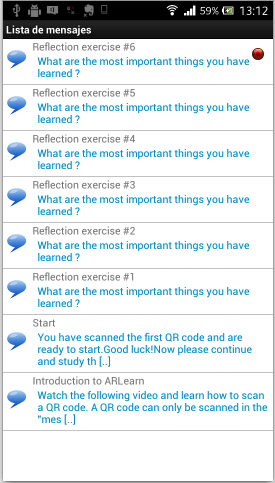
\includegraphics[width=0.3\linewidth]{img/notif_fig5a}
		\label{fig:notif_5a}
	}
	\subfloat[Tip \#11 collected by a participant from group A prompted to reflect and externalize knowledge in audio speech recording]{
		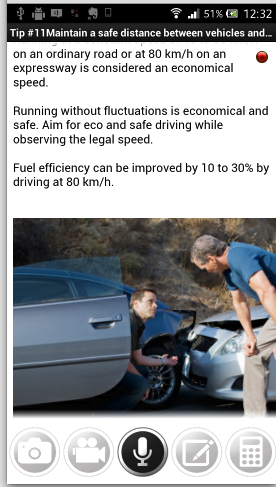
\includegraphics[width=0.3\linewidth]{img/notif_fig5b}
		\label{fig:notif_5b}
	}	
	\subfloat[Notification prompting users to reflect. Users from group B had to externalize knowledge. Users from group C did not]{
		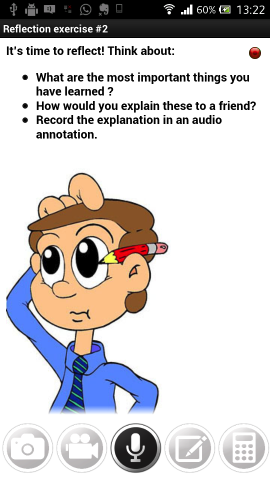
\includegraphics[width=0.3\linewidth]{img/notif_fig5c}
		\label{fig:notif_5c}
	}	
      \caption{Formative study. Notifications fostering reflective practice on-action}
      \label{fig:notif_5}
\end{figure}
\end{center}
\subsection{Results}
\subsubsection{Reflecting in-action with mobile notifications}

\begin{table}[h]
  \centering
  \small
  \caption{Overall Means (M), Standard Deviations (SD) and reliability coefficient ($\alpha$ = Cronbach�s Alpha) for ''intrinsic motivation'' subclass. 7-point likert. (*Interest is considered self-report message of intrinsic motivation)}
  \label{tbl:notif_table4}

\begin{tabular}{lllll}
\thickhline
\textbf{Subscale} 	
	& \textbf{M(SD)} 
	& \multicolumn{1}{l}{\textbf{\begin{tabular}[c]{@{}l@{}}$\alpha$\end{tabular}}}	
	& \textbf{Sample item} \\ \thickhline
\multicolumn{1}{l}{\textbf{\begin{tabular}[c]{@{}l@{}}Interest*\end{tabular}}}		
	& 4.70(1.49)	
	& .86			
	& \multicolumn{1}{l}{\begin{tabular}[c]{@{}l@{}}I enjoyed doing this activity very much\end{tabular}} \\	
\multicolumn{1}{l}{\textbf{\begin{tabular}[c]{@{}l@{}}Competence \end{tabular}}}		
	& 4.12(1.37)	
	& .85			
	& \multicolumn{1}{l}{\begin{tabular}[c]{@{}l@{}}I think I am pretty good at this activity\end{tabular}} \\
\multicolumn{1}{l}{\textbf{\begin{tabular}[c]{@{}l@{}}Pressure \end{tabular}}}		
	& 2.29(1.47)      
	& .83			
	& \multicolumn{1}{l}{\begin{tabular}[c]{@{}l@{}}I felt very tense while doing this activity\end{tabular}} \\
\multicolumn{1}{l}{\textbf{\begin{tabular}[c]{@{}l@{}}Usefulness\end{tabular}}}		
	& 4.88(1.50)      
	& .87			
	& \multicolumn{1}{l}{\begin{tabular}[c]{@{}l@{}}I believe this activity could be of some value to me\end{tabular}}	\\ \hline
\end{tabular}

\end{table}

The Cronbach's alpha coefficient concluded in reliable values for all the IMI variables ranging from .83 to .87 (See Table \ref{tbl:notif_table4}). Calculating the overall mean in the variables of intrinsic motivation resulted in higher values for group C in contrast to the lower values for group A. Table \ref{tbl:notif_table5} illustrates the answers clustered into its four variables. On the one hand, group C resulted in higher values for \textit{interest} and \textit{competence}, group B resulted in higher values for \textit{pressure}, and group A resulted in higher values of \textit{usefulness}. On the other hand, group A resulted in the lower values for \textit{interest}, \textit{competence} and \textit{pressure}. Group C resulted in the lower values for usefulness.
\begin{table}[h]
  \centering
  \small
  \caption{Group-clustered measures for \em intrinsic motivation \em variables}
  \label{tbl:notif_table5}
\begin{tabular}{lllll}
\thickhline
\textbf{ } 		& \textbf{Group A} 	& \textbf{Group B} 	& \textbf{Group C} \\ 
\textbf{ } 		& \textbf{M(SD)} 	& \textbf{M(SD)} 	& \textbf{M(SD)} \\ \thickhline
\textbf{Interest}	& 4.56(1.54)		& 4.66(1.44)				& 4.87(1.51)          \\ 
\textbf{Competence} & 3.99(1.37) 		& 4.08(1.33)				& 4.30(1.41)         \\ 
\textbf{Pressure}	& 2.26(1.54)        & 2.35(1.34)				& 2.28(1.55)          \\ 
\textbf{Usefulness}	& 4.95(1.56)        & 4.88(1.57)				& 4.85(1.37)          \\ \hline
\textbf{Overall}	& 3.94(1.79)        & 3.99(1.70)				& 4.08(1.77)          \\ \hline

\end{tabular}
\end{table}
Knowledge was measured upon the number of correct answers in the 15-items questionnaire. Table \ref{tbl:notif_table6} illustrates mean and standard deviations values for the three different treatments. The experiment resulted in higher mean values for group C in contrast to group B that resulted in lower mean values.
\begin{table}[h]
  \centering
  \small
  \caption{Group-clustered measures for  \em knowledge \em variable. 15 (right/wrong) questions}
  \label{tbl:notif_table6}
\begin{tabular}{lllll}
\thickhline
\textbf{ } 		& \textbf{Group A} 	& \textbf{Group B} 	& \textbf{Group C} \\ 
\textbf{ } 		& \textbf{M(SD)} 	& \textbf{M(SD)} 	& \textbf{M(SD)} \\ \thickhline
\textbf{Knowledge}	& 11.25(1.71)		& 10.65(1.59)				& 11.55(1.46)          \\ \hline
\end{tabular}
\end{table}
An analysis of variance (ANOVA) was performed with the aim to identify differences between means and their variation among the groups. As illustrated in figure \ref{fig:notif_6}, the ANOVA test resulted in non-significant values (Pr(>F) > 0.05) for IMI variables. Nevertheless, the ANOVA test resulted in a remarkable variation in \em knowledge  \em for group C with respect to the other groups.

The results obtained in the ANOVA test for the variable of \textit{knowledge} show differences that cannot be assured to be determinant.

When the participants had finished the activity, they were offered the possibility to provide open feedback by answering to the question \textit{''how was the learning experience?''}. This interview raised the following insights to be taken into account:
\begin{enumerate}
\item Combining multiple devices is not always well accepted. A participant from group C (\#42) reported that \textit{''the only effect from the mobile device was to disturb and disrupt my learning experience''}. Similar, \#44 from group C reported that \textit{''when I am focused on reading, receiving messages is more disruptive than helpful''}. Participant \#29 reported that \textit{''asynchronous notifications were annoying since they came in the middle of the reading and I had to stop reading the eBook, to open the incoming notification in the mobile device''}.
\item Participants self-organized their reading approaching the sections of the book depending on the type of multimedia formats. This eBook contained texts, pictures, videos and audios distributed among the fifteen hints. E.g. participant \#33 reported that she had first read the text from the eBook and after that watched the sequence of videos. Participants from group A adopted different behaviours when reading the eBook. As the participants of this group were assigned to scan, collect and reflect on their six preferred hints, some participants decided to scan (on the go) as they were advancing on the book. Others decided to read the whole book first, and then sequentially scan, collect and reflect on their preferred set of items.
\item Iterating notifications with the same content produces a drastic polarization of user�s interest on the notification. Some users from groups B and C reported that after the second notification they gave up reading when they noticed every notification contained the same instruction (\#12, \#42). 
\item Participants that were aimed to self-reflect and not actively externalize the audio speech on the mobile device (group C) sometimes skipped to perform the self-reflection exercise. The fact that participants from group C were not prompted to record the exercise of reflection resulted in less disrupted readings for this group. Participant \#30 \textit{''after the second notification, as I was not asked to actively do something I did not reflect and kept on reading''}.
\end{enumerate}
\begin{figure}
     \centering
     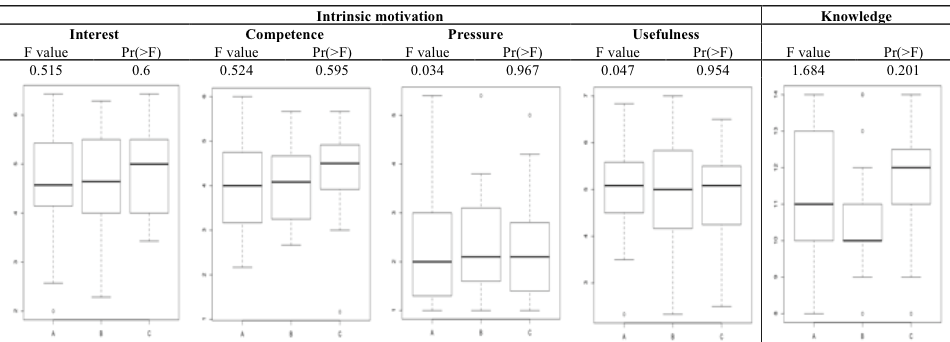
\includegraphics[width=1\linewidth]{img/notif_fig6}
     \caption{Results from the ANOVA test}
     \label{fig:notif_6}
\end{figure}
   
\section{Discussion and conclusions}
This chapter has explored the use of mobile notifications to foster reflection on learning by presenting the results of two studies that involved 97 participants in total. Mobile notifications have been used to support users in the competence of \textit{learning to learn}  \citep{EuropeanCommission2007} raising reflection and awareness as trigger to foster understanding (meta-learning) \citep{Biggs1985} and motivation on learning.

The formative study provides an instantiation in which smartphones are used to stimulate meta-learning about the common life as a learner. A proportion of pupils accepted and was able to use their personal smartphone for "serious" messages coming from the researcher outside the school hours. Whilst it can seem obvious, this precondition does not speak for itself. \cite{Hardy2008} show that even when undergraduates do have a good level of IT competence and confidence, they tend to be conservative in their approaches maintaining a clear separation between technologies for learning and for social networking. On the other hand, \cite{Jones2008} report that, despite being unaccustomed to using their mobile phones for academic study, students willingly accepted SMS reminders focused on time management and not on learning consolidation from their tutor via a bulk texting service. Nevertheless, subsequent identical notifications prompting the student to reflect are not well accepted. This observation can be concluded not only from the results of the decreasing rate of participation in the first study, but also in the second experiment in which participants reported not paying attention to succeeding notifications when they noticed that the first two were identical. Hence the effects of subsequent non-identical notifications should be explored in further investigation.

This study suggests that learners willing to stop and think about \textit{''how''} and \textit{''what''} they learn, still perceive the school as the major channel of learning. These reports contrast with the ones from users that voluntarily decided not to take part in the daily reflective exercise in which the majority of them perceived Internet as the main channel of learning. Indeed, schools� monopoly over learning processes seems to be challenged by the emergence of a rich ecosystem outside school walls as heralded by the Internet (Table \ref{tbl:notif_table1}). Of particular concern for future research is to ascertain how school and other channels of education contribute to youth�s intellectual growth \citep{Facer2011}. In such an investigation, student�s voice is obviously critical. And to express it, young people will have to learn to think as learners in order to provide valuable accounts of what they are living as learners in multiple contexts. This need to be able to reflect on the common life as learners takes us back to the what motivated this study: defining methods and designing tools to make learning an object of attention and reflection. 

Three findings emerge from the formative study regarding reflective practice in students� common life: 

\begin{enumerate}
\item There is no anchored habit of the students to see themselves as learners and to develop a \textit{''professional''} awareness (see section \textit{Familiarity with reflective practice}) about their daily activity/job at school \citep{Ertmer1996,Sternberg1998} and the learning opportunities after school. This study demonstrates that notifications instantiated in personal mobile devices can be used by secondary school students to make them focus and reflect on their autobiography as a learner. These signals and the subsequent reflection moments are expected to trigger actions from student's side towards the development of an identity as a learner. From the authors� perspective, there are two main factors in the design of mobile notifications that positively contribute to foster reflection: first, the personal mobile device is perceived by students as an intimate channel in which they have the privacy to deal with meta-learning aspects beyond the content being learned; second, in contrast to traditional orientation-talks from teachers or parents, the fact that students know that notifications are coming from an external non-usual source (researchers) makes them focus more intensively on the offer to reflect;
\item Providing time to perform reflective activities on this topic is appreciated by about half of the participants (see section \textit{Appreciation of reflective practice}) for reasons relating to sense-making and professional development as a student. Notifications prompting to reflect seem to be effective when they are received at the end of the day (8pm) so that students can make one step back and think how their learning day was;
\item The stop-and-think beacons offered here are considered as useless or superfluous by a good deal of students, even when they have been designed not to last a long time (for similar attitudes of rejection of reflection see \cite{Watkins2001,Johnson2009}). The fact that the content of the notifications delivered for every iteration was always the same, as well as the fact that the notifications were received always at the same time of the day (8pm) could increase the perception of superfluousness. Further research must be done on how these notifications are perceived when both the content and the delivery time are not (so) predictable.
\end{enumerate}
Overall these findings contribute to understanding the basic notions of learning, self-reflection and the use of triggers from mobile devices in the context of a formal educational institution. The convergence of information, communication and broadcasting technologies is one of the major determinants of the need for lifelong learning \citep{Longworth2013}. Both studies presented in this chapter provide relevant insights on the use of technology to foster key competences for lifelong learning  \citep{EuropeanCommission2007}: \textit{digital competence } by combining the use of mobile devices and tablets for meta-learning; \textit{learning to learn} by providing users new channels to reflect on their learning.

The formative study shows that simplistic instantiations of notifications via SMS are useful to promote reflective practice on the learning activities scattered throughout the day (reflection on-action \citep{Schon1983}). 

The second experiment implements one step forward in the complexity of the notifications by combining the use of different devices and interactions to reflect in-action. Our assumption was that the group with the highest number of interactions (group A), using user-triggered notifications combined with the externalization of knowledge and the collection of learning objects, would result in increased values for knowledge and motivation. 

The results obtained in the experimental study suggest that asynchronous notifications prompting users to reflect are not well accepted while multitasking with another learning activity. Automatic notifications resulted in disruptive learning experiences where few participants found an added value to this treatment. In contrast, participants were able to customize their learning experience by adapting the order to read, reflect and externalize when the notifications should be delivered (scanning the QR code).  In fact, none of the participants reported that user-launched notifications were a cause of disruptive learning experiences. This finding reinforces the outcome from our previous study where participants preferred to receive user-triggered (event-based) notifications to \textit{''stop and think''}, in contrast to asynchronous notifications \citep{TabuencaCAA2014}. Measures of knowledge and intrinsic motivation resulted in non-significant differences between the group that approached user-launched notifications (group A) and the groups that approached automatic notifications (groups B and C).

The fifth research question of this chapter aimed to gain insight on whether the externalization of knowledge using audio speech recordings on a mobile device (groups A and B) would result in increased values for knowledge and motivation compared to the participants that did not do it.  This was not the case since differences between the groups were not significant. Contrary, the results presented above only put forward for consideration that within the group of participants that received the same type of notifications (groups A and C with scheduled-based notifications), the participants that did not externalize knowledge (group C) could score better in this variable. This finding confirms some previous insights on the limitations of \textit{''thinking aloud''} to understand learning \citep{Young2009} pinpointing to issues of participant's reactivity, participant's verbal abilities, and whether the information provided by think-aloud accurately reflects thinking. In our specific case, we can add \textit{digital competence } as one more limitation in the fact that participants had to deal with both a non-familiar app and smartphone to externalize their reflections. The interviews after the experiment confirmed this disruption where some of the participants reported not to be used to this smartphone model (Sony Xperia), the operating system (Android 4.01), or the mobile app (ARLearn \citep{Ternier2013}). \cite{Wilson1994} states that \textit{''while it is not claimed that think aloud provides a complete insight into the human mind, it certainly is a useful tool available to the researcher''}. The results obtained in this experiment are inconclusive and do not confirm that externalizing the knowledge on mobile devices might be beneficial towards better motivation and knowledge. Nevertheless, we strongly believe that this negative effect was caused by the fact that participants had to deal with a non-familiar environment to record their audio (See fig. \ref{fig:notif_5b} and \ref{fig:notif_5c}). Hence, participants lost the focus on what they were reading while handling the mobile tool to externalize the reflection exercise. In the future we suggest further research on the benefits and limitations of thinking aloud providing tools that are familiar to the participants so they can naturally record an audio without losing the thread on what the user had learnt.

The last research question is built upon the assumption that the reflection preceding the collection of a learning object awakes a motivation on the learning topic. Some participants highlighted the usefulness of collecting the hints on energy-efficient driving to be further read and studied in more detail when they had time. Nevertheless, this is not the focus of this study. Measures of knowledge and intrinsic motivation resulted in non-significant differences between the group that collected learning objects and the groups that did not. There is a need to quantify whether the reflection that precedes the collection of learning objects has an impact on learning in further research.

The sample in the formative study decreased for technical reasons but also for reasons probably tied to the importance granted to reflection. These reasons should be investigated for themselves and a subsequent study should be carried out with bigger samples. This study also prompted students only four times. More investigation is needed into the tension of intruding into the pupils' out-of-school time. It has already been shown that many university students do not like their academic studies to intrude into personal time or their social networking activities. 

The answers reported in the interview of the experimental study point to differences between users with regard to familiarity with mobile technologies (\textit{digital competence} \citep{EuropeanCommission2007}). In this scenario, users who were not so agile interacting with devices, were more focused on the mobile interaction than on the reflection exercise itself. Likewise, the time devoted by the participants to accomplish the activity in the experimental study was quite unbalanced (even of participants with the same treatment). Some participants were faster reading the eBook so they were still receiving notifications prompting to reflect when they had completed the task. Participants with least digital competence received all the notifications when they were reading the first two pages of the book. Hence, this experiment uncovers familiarity with the tools as one of the main limitations to accomplish seamless learning experiences. We also highlight the short duration (one hour per user) of the learning experience, and the high frequency of the notifications received during the experiment as limitations of this study. We suggest further research on the effects of notifications in longitudinal studies when they are received in personal mobile devices.

These results relight the need for support in Mobile Seamless Learning (MSL) experiences \citep{Wong2011d}, in particular, the combined use of multiple device types (MSL7), seamless switching between multiple learning tasks (MSL8) (such as data collection, analysis and communication), encompassing formal and informal learning (MSL1) and knowledge synthesis (MSL9). 




